\section{Network Layer Architecture}

The network layer acts as the control plane of the proposed LoRa-based V2V mesh system. We designed it as a
portable, hardware-independent core that sits between the application services and the radio-facing
transmission services. Its job is to take locally generated safety data and turn it into network frames that
can be disseminated, to check received frames against the propagation policy, and to control rebroadcasting so
that reliability improves without wasting channel time. We do this by keeping clear boundaries that separate
forwarding logic from platform-specific communication and sensing details, so the same network behavior can be
used on embedded devices and in a host-side simulation.

At the transmission boundary, each outgoing frame is a fixed network header followed by application payload
bytes. The header carries message identity, temporal validity, origin context, per-hop transmitter context, and
propagation constraints, so downstream nodes can decide what to do based on self-contained metadata. Using a
fixed header length keeps parsing deterministic and the overhead bounded. The payload limit is set based on the
LoRa frame-size ceiling, so any generated frame is admissible for the physical channel. A unique message
identifier is created by combining the source identity with a local sequence progression. This supports replay
suppression and idempotent handling across multi-hop dissemination.

A key design principle is separating immutable origin metadata from mutable per-hop transmitter metadata.
Origin metadata does not change for the lifetime of a message and represents the initial source state at the
time of creation. Transmitter metadata is updated at every relay and represents the most recent forwarding
node. This separation lets the forwarding logic reason about the overall propagation intent and the local
progress at the same time, which is needed for hold-back scheduling and redundancy suppression in dynamic
vehicular topologies.

Operationally, the data plane has two coordinated paths: synchronous origination and asynchronous
reception-driven forwarding. During origination, the layer checks that the payload is admissible, builds the
network header using local time and mobility context, records the message identity in a duplicate-tracking
structure, and sends a single broadcast frame. During reception, incoming frames are first buffered in a
bounded event queue and then processed by worker execution contexts that handle parsing, policy evaluation,
local delivery, and (if needed) relay scheduling. This separation stops the receive callbacks from becoming
policy bottlenecks and makes the timing more predictable under bursty traffic. The receive-path processing
sequence is shown in Fig.~\ref{fig:network-layer-sequence}.

\begin{figure*}[!t]
\centering
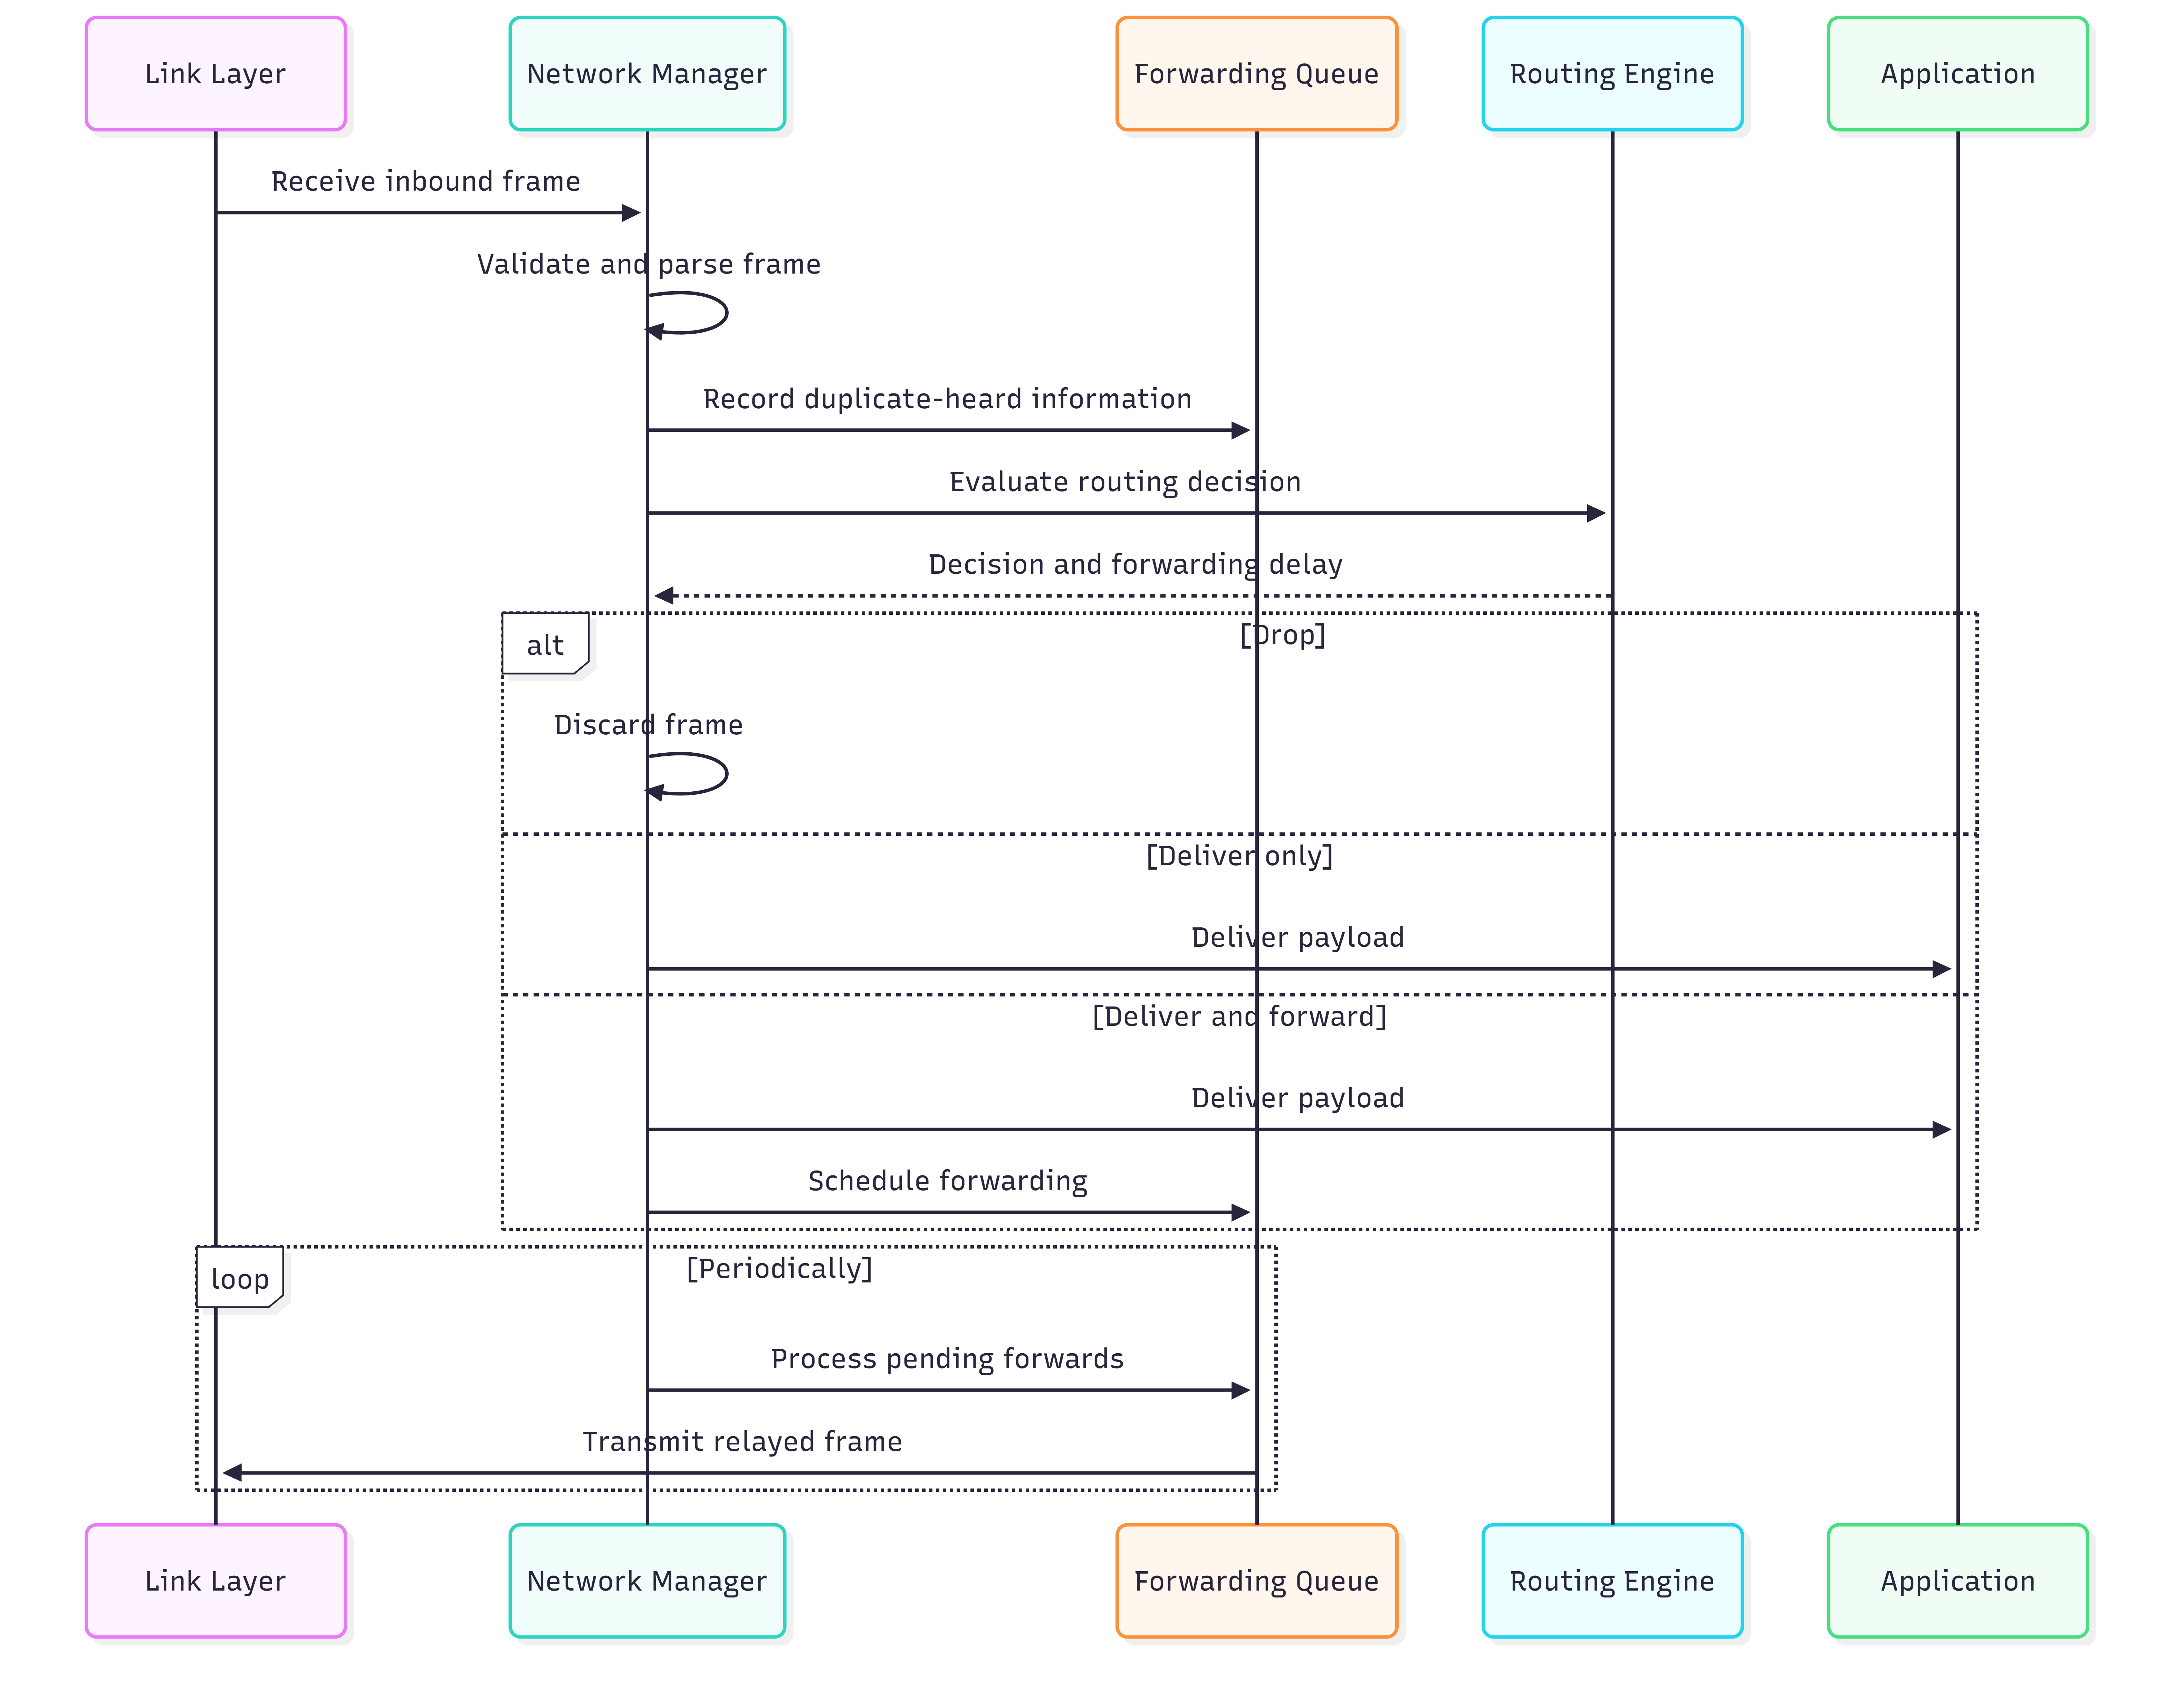
\includegraphics[width=0.95\textwidth]{assets/architecture/Network_layer_seq.png}
\caption{Receive-path sequence of network-layer processing, from link-layer callback ingestion and queueing to
routing evaluation, local delivery, and deferred forwarding.}
\label{fig:network-layer-sequence}
\end{figure*}

Forwarding decisions are made using an ordered evaluation pipeline that prioritizes safety and bounded
propagation. Frames are first screened for temporal expiry, replay status, and remaining hop budget. After
that, we check distance-constrained dissemination and directional eligibility when directional propagation is
requested. Messages that pass these gates become relay candidates, and we assign them a deferred forwarding
delay instead of retransmitting immediately. The delay is computed from a composite estimate of path progress
and link quality, and then adjusted by traffic priority so urgent safety traffic propagates with lower latency
while less critical traffic is naturally delayed. This mechanism implements contention-aware spatial diversity
by encouraging favorable relays to transmit earlier and discouraging simultaneous redundant rebroadcasts. The
ordered decision logic and outcomes are summarized in Fig.~\ref{fig:network-layer-decision}.

\begin{figure*}[!t]
\centering
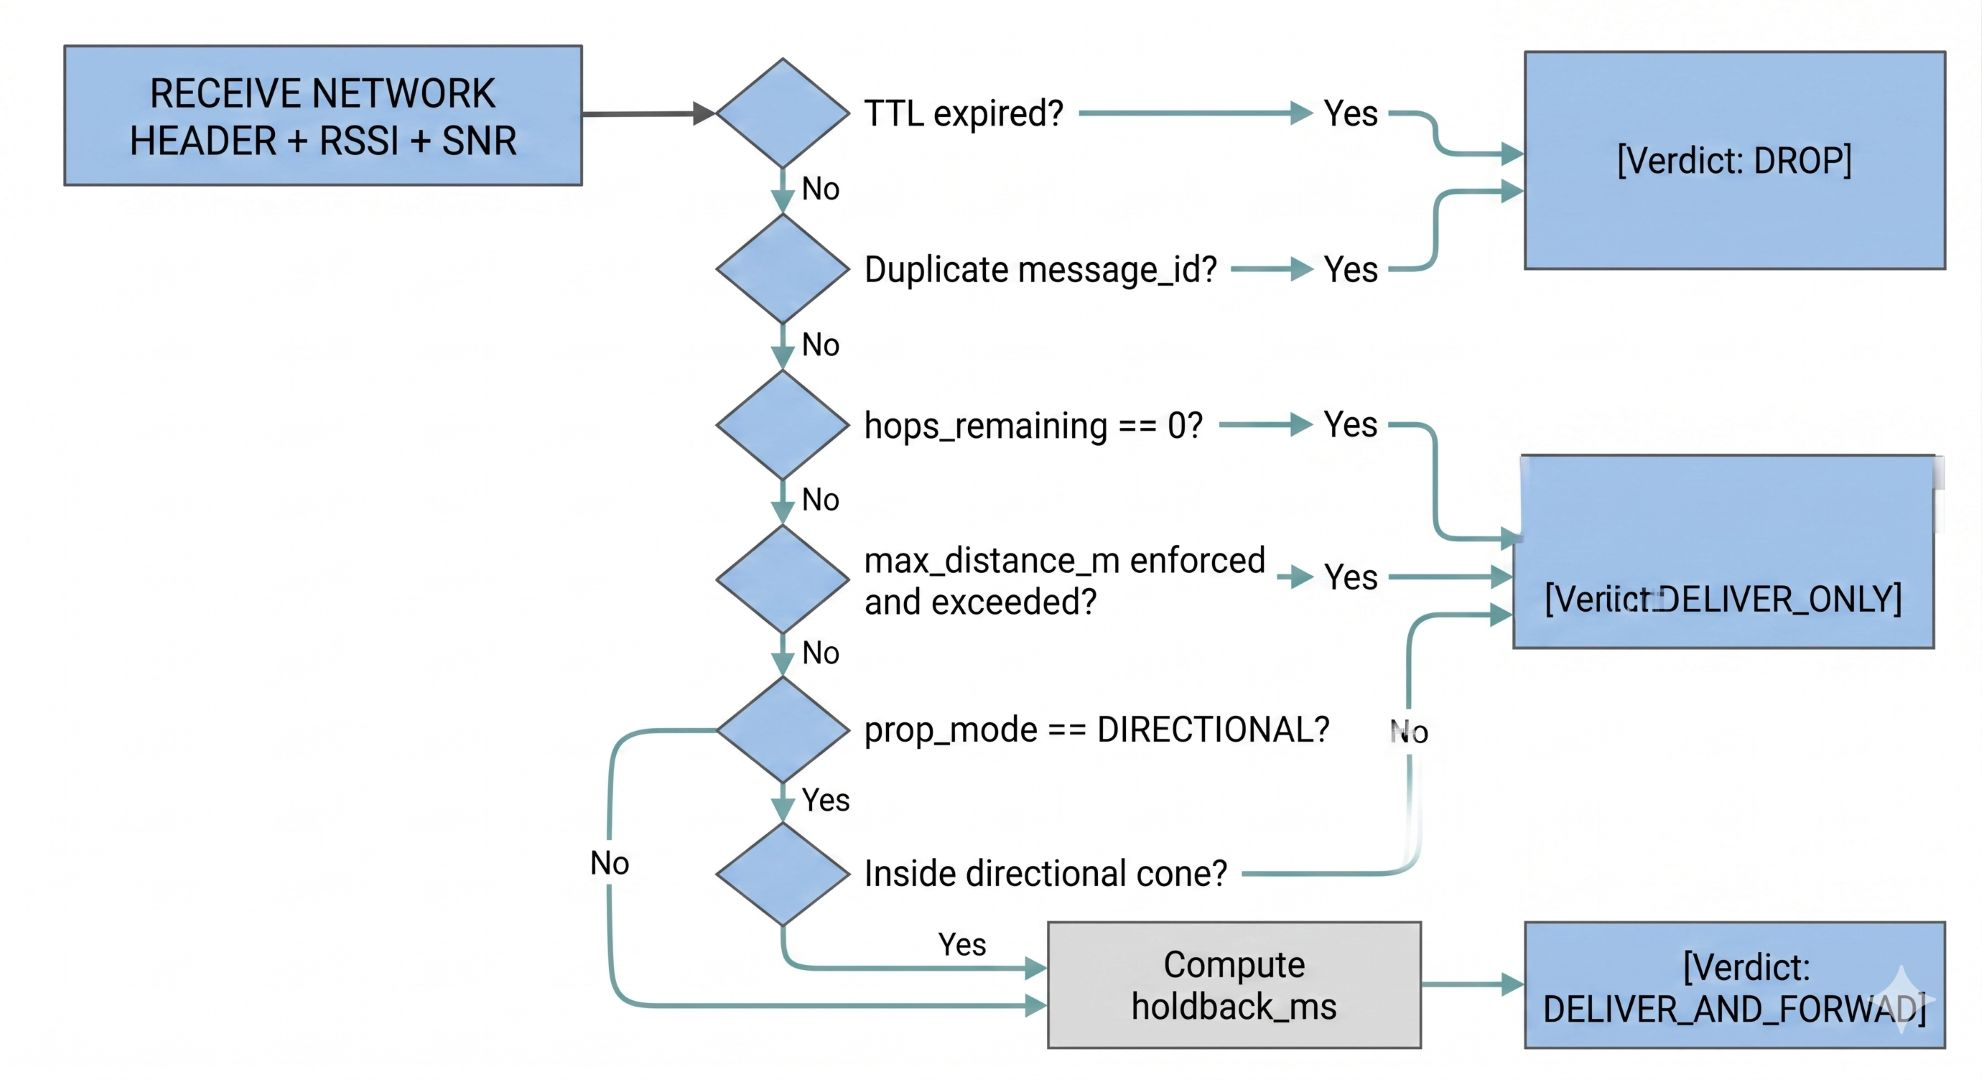
\includegraphics[width=0.6\textwidth]{assets/architecture/network_layer_decision.jpg}
\caption{Network-layer decision pipeline for received frames, showing the ordered checks that determine drop,
deliver-only, or delayed forwarding outcomes.}
\label{fig:network-layer-decision}
\end{figure*}

To further limit broadcast redundancy, the architecture uses two suppression mechanisms. First, duplicate
filtering stops repeated processing and forwarding of message identities that have already been seen. Second,
queued relays can be canceled if later overheard transmissions suggest that upstream progression already
covered what this node would have contributed. This geometric suppression reduces unnecessary retransmissions
without explicit coordination exchanges, which fits bandwidth-constrained and intermittently connected
vehicular channels.

Concurrency management is important for correctness. The network layer uses separate execution contexts for
receive-path processing and timer-driven relay emission, with mutex- and condition-variable-based
synchronization around bounded shared queues and callback handoff state. Lifecycle control is made robust for
repeated start-stop operation, with deterministic initialization, safe termination of background activity, and
clean release of receive handlers during shutdown. Overall, this threading model keeps a clear separation
between ingress handling, routing computation, and deferred transmission timing.

The architecture also exposes bounded configuration controls for duplicate-cache capacity, relay-queue
capacity, receive-queue depth, and forwarding delay limits. These parameters define the operational envelope
for memory consumption, latency, and admission behavior, and they allow systematic trade-off analysis between
responsiveness and channel load. Along with fixed frame-level constraints, this configuration model helps keep
runtime behavior predictable across different hardware targets.

Finally, we embed the same network-layer core in a deterministic simulation runtime to support repeatable
validation under controlled mobility and channel conditions. Each simulated node runs the same logical network
functionality as a deployed node, while a shared virtual clock and event-driven channel model control
transmission timing, reception outcomes, and channel impairments. Since routing and forwarding semantics are
preserved across deployment and simulation, the behavior observed in the lab can be transferred more directly
to field-oriented configurations.

